\documentclass[11pt, letterpaper, onecolumn, oneside, final]{article}

\usepackage{basic}
\usepackage [autostyle, english = american]{csquotes}
\MakeOuterQuote{"}
\usepackage{graphicx}

\begin{document}
\begin{center}
\section{Thonny Installation \& Pointers}
\end{center}

\section{Installation:}
\begin{enumerate}
\item Go to \textcolor{blue}{\underline{https://thonny.org}} and download the installer for your operating system, be it Mac or Windows.
\item Run the installer, clicking "Continue" or "Accept" whenever prompted.
\end{enumerate}


\section{How to use Thonny:}\\
\\
\begin{center}
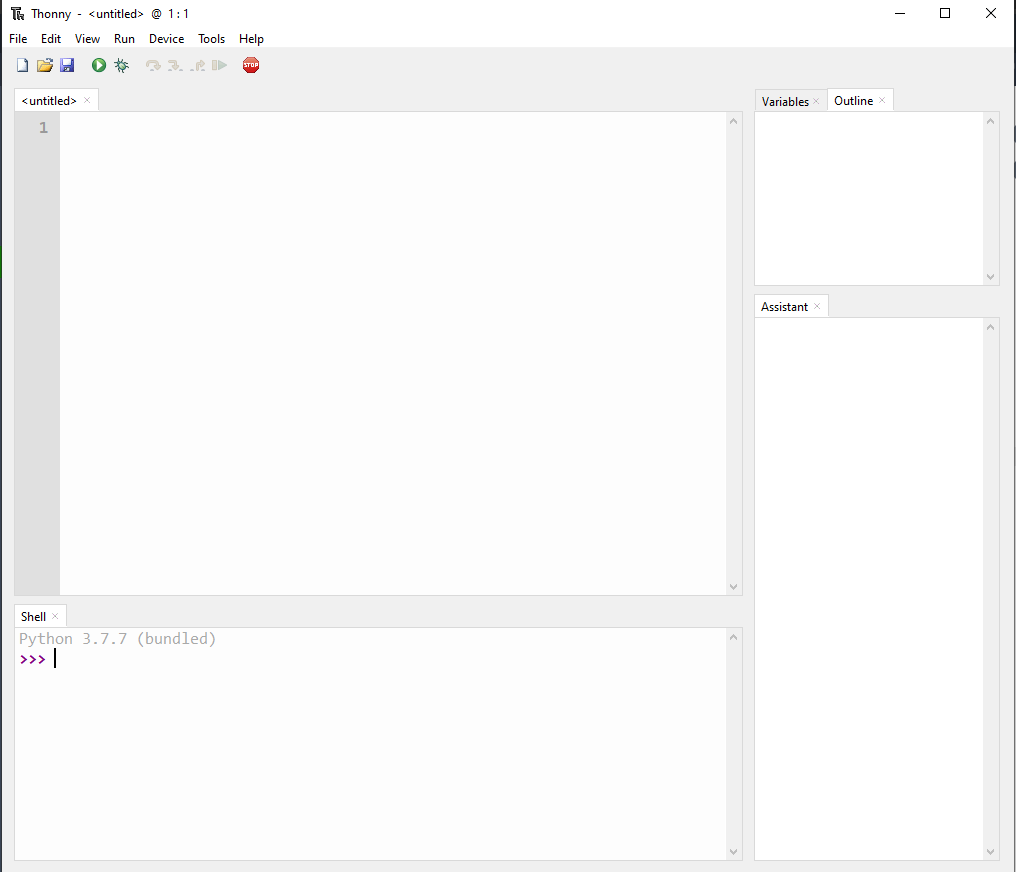
\includegraphics[scale=.3]{thonny}
\end{center}
\begin{enumerate}
\item This is your Thonny window. It has an Editor, a Shell, and an Assistant to help you understand errors. This is what you will be using to create and run your code all semester.
\item Go to View in the top left, and then make sure "Assistant" and "Shell" are selected.
\begin{center}
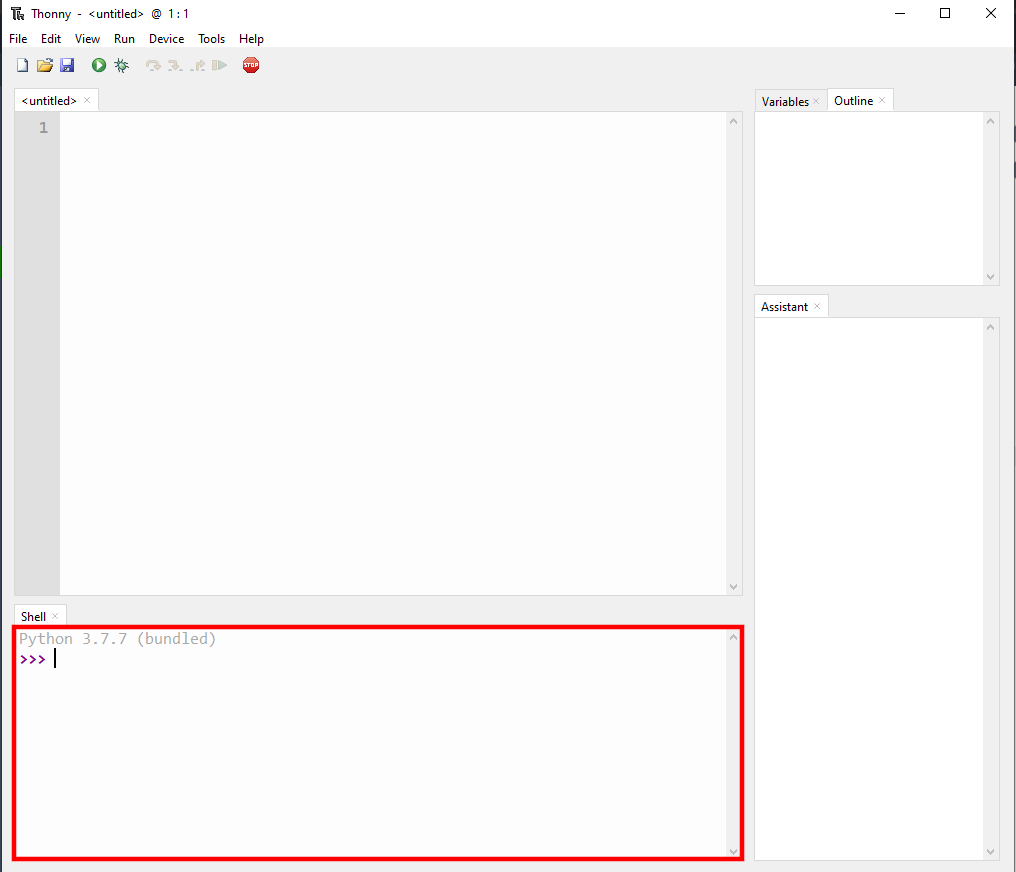
\includegraphics[scale=.3]{thonny_interpreter}
\end{center}
\item The Shell window is highlighted in red. Shell is where your code will be run and output will be displayed. It can also be used to run things in the Python interpreter.
\begin{center}
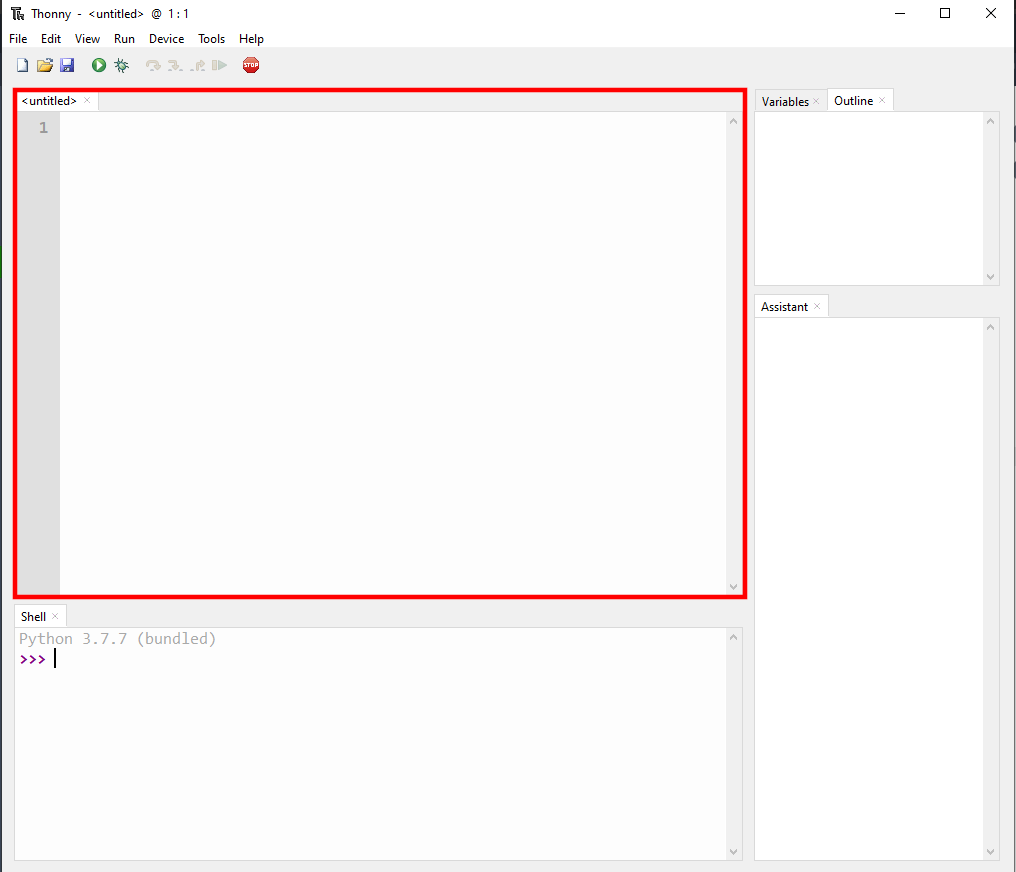
\includegraphics[scale=.3]{thonny_editor}
\end{center}
\item The Editor is where you can edit files, write your programs, and work on projects & labs.
\begin{center}
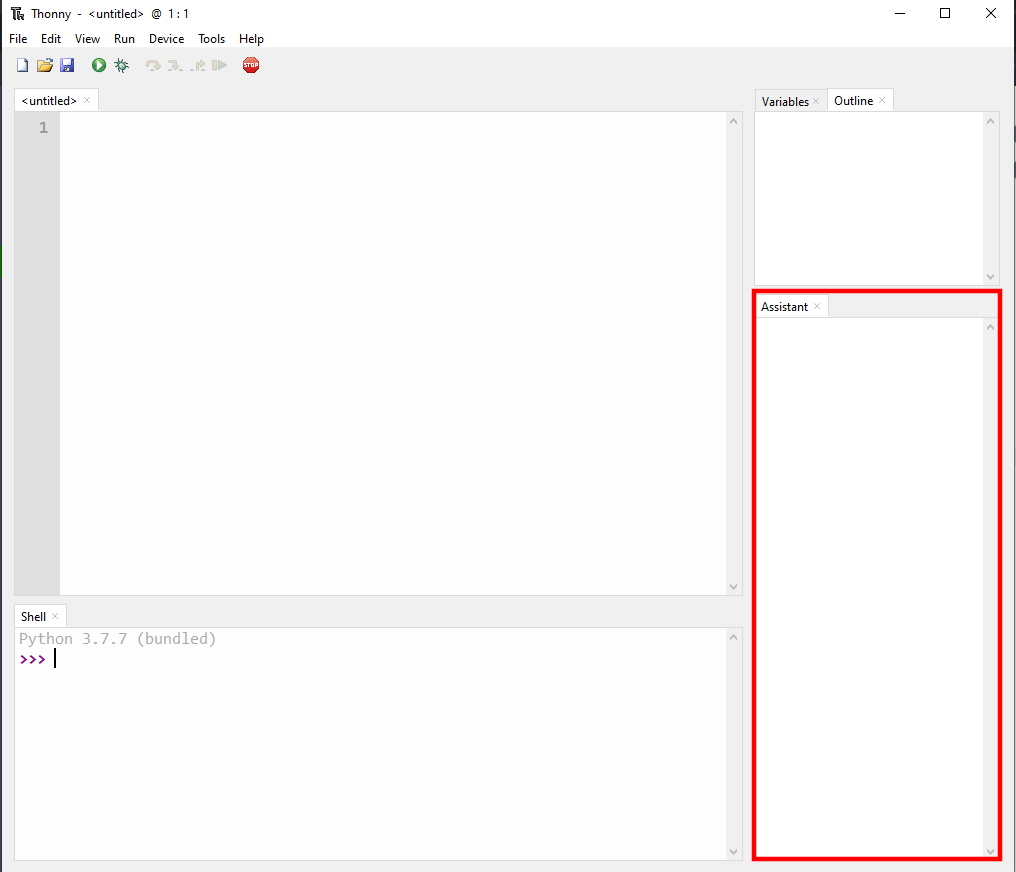
\includegraphics[scale=.3]{thonny_assistant}
\end{center}
\item The Assistant shows you details about various errors and issues in your code, which you can use to help you with debugging. 
\begin{center}
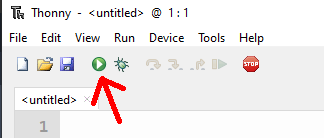
\includegraphics[scale=.7]{thonny_run}
\end{center}
\item Click the green "Run" button (or press F5) to run the program currently being edited. If you ever need to stop your program's execution for whatever reason, you can also press the red "Stop" button to the right. 
\end{enumerate}
\end{document}